\documentclass[answers]{exam}\newcommand{\repositoryInformationSetup}{     \usepackage[dvipsnames]{xcolor}     \usepackage[ angle=90, color=black, opacity=1, scale=2, ]{background}      \SetBgPosition{current page.west}      \SetBgVshift{-4.5mm}      \backgroundsetup{contents={{\color{green}\texttt{-{}-} differs from commit \texttt{40a9b87} in 0 files}}} } \newcommand{\commit}{{{\color{green}40a9b87}}}\usepackage{amsmath}
\usepackage{xspace}
\usepackage{bbm}
\usepackage{ifthen}


\newcommand{\secref}[1]{Sec.~\ref{sec:#1}}
\newcommand{\Secref}[1]{Section~\ref{sec:#1}}
\newcommand{\appref}[1]{App.~\ref{sec:#1}}
\newcommand{\Appref}[1]{Appendix~\ref{sec:#1}}
\newcommand{\tabref}[1]{Tab.~\ref{tab:#1}\xspace}
\newcommand{\Tabref}[1]{Table~\ref{tab:#1}\xspace}
\newcommand{\figref}[1]{Fig.~\ref{fig:#1}\xspace}
\newcommand{\Figref}[1]{Figure~\ref{fig:#1}\xspace}
\newcommand{\Eqref}[1]{Equation~\ref{eq:#1}\xspace}
\def\Ref#1{Ref.~\cite{#1}} \newcommand{\Reference}[1]{Reference~\cite{#1}}
\newcommand{\Refs}[1]{Refs.~\cite{#1}}
\newcommand{\References}[1]{References~\cite{#1}}



\newcommand{\issue}[1]{\href{\repoURL/issues/#1}{Issue #1}}
\newcommand{\pullrequest}[1]{\href{\repoURL/pulls/#1}{Pull Request #1}}



\newcommand{\arxiv}[1]{\href{http://www.arxiv.org/abs/#1}{arXiv:#1}}



\newcommand{\goesto}{\ensuremath{\rightarrow}}
\newcommand{\infinity}{\infty}
\newcommand{\Integers}{\mathbb{Z}\xspace}
\newcommand{\integers}{\Integers}
\newcommand{\one}{\ensuremath{\mathbbm{1}}}
\newcommand{\order}[1]{\ensuremath{\mathcal{O}\left(#1\right)}\xspace}
\newcommand{\Rationals}{\mathbb{Q}\xspace}
\newcommand{\Reals}{\mathbb{R}\xspace}
\newcommand{\Complexes}{\mathbb{C}\xspace}
\newcommand{\union}{\ensuremath{\cup}}
\DeclareMathOperator{\erf}{erf}
\newcommand{\laplace}[1]{\ensuremath{\mathcal{L}\left\{#1\right\}}\xspace}
\newcommand{\inverselaplace}[1]{\ensuremath{\mathcal{L}\inverse\left\{#1\right\}}\xspace}


\DeclareMathOperator{\odd}{odd}
\DeclareMathOperator{\even}{even}
\DeclareMathOperator{\sinc}{sinc}
\DeclareMathOperator{\real}{Re}
\DeclareMathOperator{\imag}{Im}





\DeclareMathOperator{\sech}{sech}
\DeclareMathOperator{\csch}{csch}
\DeclareMathOperator{\arccosh}{arccosh}
\DeclareMathOperator{\arcsinh}{arcsinh}
\DeclareMathOperator{\arctanh}{arctanh}
\DeclareMathOperator{\arcsech}{arcsech}
\DeclareMathOperator{\arccsch}{arccsch}
\DeclareMathOperator{\arccoth}{arccoth}



\DeclareMathOperator{\arcsec}{arcsec}
\DeclareMathOperator{\arccot}{arccot}
\DeclareMathOperator{\arccsc}{arccsc}



\newcommand{\oneover}[1]{\ensuremath{\frac{1}{#1}}}                             \newcommand{\inverse}{\ensuremath{^{-1}}}                                       \providecommand{\half}{\ensuremath{\frac{1}{2}} }                               \renewcommand{\half}{\ensuremath{\frac{1}{2}} }                                 \newcommand{\quarter}{\ensuremath{\frac{1}{4}} }                                



\newcommand{\dd}[3][1]{
    \ifthenelse { \equal {#1} {1} }
                {\ensuremath{\frac{d#2}{d#3}}}
                {\ensuremath{\frac{d^{#1}#2}{d#3^{#1}}}}
    }

\newcommand{\pp}[3][1]{
    \ifthenelse { \equal {#1} {1} }
                {\ensuremath{\frac{\partial#2}{\partial#3}}}
                {\ensuremath{\frac{\partial^{#1}#2}{\partial#3^{#1}}}}
    }

\newcommand{\ppp}[3]{\ensuremath{\frac{\partial^2#1}{\partial#2\,\partial#3}}}

\providecommand{\id}{}
\renewcommand{\id}[1]{\ensuremath{\; \mathrm{d}#1}}

\newcommand{\abs}[1]{\ensuremath{\left| #1 \right|}\xspace}
\newcommand{\magnitude}{\abs}
\newcommand{\average}[1]{\ensuremath{\left\langle #1 \right\rangle}\xspace}

\newcommand{\ket}[1]{\ensuremath{\left|\;#1\;\right\rangle}}
\newcommand{\bra}[1]{\ensuremath{\left\langle\;#1\;\right|}}
\newcommand{\bracket}[2]{\ensuremath{\left\langle\;#1\;\middle|\;#2\;\right\rangle}}
\let\braket\bracket




\newcommand{\identity}{\ensuremath{\mathds{1}}}
\newcommand{\diag}[1]{\ensuremath{\text{diag}\left(#1\right)}}
\newcommand{\tr}[1]{\ensuremath{\text{tr}\left[#1\right]}}
\newcommand{\transpose}{\ensuremath{{}^{\top}}}
\newcommand{\adjoint}{\ensuremath{{}^{\dagger}}}








\newcommand{\bash}{\texttt{bash}\xspace}
\newcommand{\git}{\texttt{git}\xspace}
\newcommand{\make}{\texttt{make}\xspace}
\newcommand{\mpi}{\texttt{MPI}\xspace}
\newcommand{\python}{\texttt{python}\xspace}

\let\builtinLaTeX\LaTeX
\def\LaTeX{\builtinLaTeX\xspace}
 \usepackage{amsmath,amssymb}
\usepackage{bm}
\usepackage{comment}
\usepackage{graphicx}
\usepackage[dvipsnames]{xcolor}
\usepackage{tikz}
\usepackage{tkz-euclide}
\usepackage{slashed}
\usepackage[
    colorlinks=true,
    allcolors=blue
]{hyperref}
\usepackage{tikz}
\usetikzlibrary{calc,patterns,decorations.pathmorphing,decorations.markings}
\usepackage{pgfplots}




\providecommand{\repositoryInformationSetup}{} \repositoryInformationSetup








\begin{document}

\title{Homework 10 --- PHYS373 2021}

\author{Domingues, Douglas}

\date{Due Apr 29, 2021}

\maketitle

\begin{questions}
	\section*{The Convolution}
	\question In class we showed, by direct integration, that $t^2*t = \frac{t^4}{12}$, and checked that $\laplace{t^2}\laplace{t} = \laplace{t^2*t} = \laplace{\frac{t^4}{12}}$.
	Show, by direct integration, that $t*t^2$ is also $\frac{t^4}{12}$.
	This shows one specific example of the general fact that $f*g = g*f$.

	\begin{solution}
		We want to compute $t \ast t^2$. By the definition of the convolution:

		$$t \ast t^2 = \int_0^t \tau (t-\tau)^2 \id{\tau}$$

		$$ = \int_0^t \tau (t^2 -2 t \tau + \tau ^2) \id{\tau}$$

		$$ = \int_0^t  (\tau t^2 -2 t \tau^2 + \tau ^3) \id{\tau}$$

		$$ = [\frac{\tau^2}{2} t^2 -2 t \frac{\tau^3}{3} + \frac{\tau ^4}{4}]_0^t$$

		$$ = \frac{t^4}{2} \frac{-2 t^4}{3} + \frac{t^4}{4} = \frac{6 - 8 + 3}{12} t^4 = \frac{t^4}{12}$$

	\end{solution}


	\question Suppose a garbage truck in a small town collects some material at a rate $g(t)$ ($g$ for garbage; maybe it's tons/week, or something like that).
	Let's assume that each piece of that material decays according to the function $d(t)$ ($d$ for decay).
	That is, if you start with 1 ton at time $t=0$ and don't add any, at a later time you have $d(t)$ tons of that material ($d$ is typically a decreasing function, and $d(0)=1$ because after no time the material hasn't decayed at all).

	Let's assume the garbage dump starts empty and the garbage truck arrives at the dump once a week and deposits $g(t) \Delta t$ tons of material ($\Delta t$=1 week).
	After the zeroeth week the total in the dump is $(g(0) \Delta t) d(0)$.
	After the first week, the total is composed of what was already in the dump, but now it's had one week to decay ($(g(0) \Delta t) d(1)$; plus the new material is added, $(g(1) \Delta t) d(0)$.

	\begin{parts}
		\part How much material is in the dump after the truck deposit's the second week's haul?

		\begin{solution}
			$(g(2) \Delta t) d(0) + (g(1) \Delta t) d(1) + (g(0) \Delta t) d(2)$
		\end{solution}

		\part How much after the third week's haul?

		\begin{solution}
			$(g(3) \Delta t) d(0) + (g(2) \Delta t) d(1) + (g(1) \Delta t) d(2) + (g(0) \Delta t) d(3)$
		\end{solution}

		\part You don't have to write anything for this part, but convince yourself that after $n$ weeks the dump contains
		\begin{equation}
			\text{total material} = \sum_{w=0}^{n} g(w) d(n-w) \Delta t
		\end{equation}
		(you can use this to check you answer to the previous two parts).

		\begin{solution}
			Makes sense. Here's the sum for week 3:

			$$ \text{total material} = \sum_{w=0}^{3} g(w) d(3-w) \Delta t $$
			$$ =  (g(0) \Delta t) d(3) + (g(1) \Delta t) d(2) + (g(2) \Delta t) d(1) + (g(3) \Delta t) d(0)$$
		\end{solution}

		Suppose instead of a small town with a garbage truck, your dump services the New York Department of Sanitation.  So, instead of garbage arriving once a week, garbage arrives at the dump continuously at a rate $g(t)$.  Convince yourself (you don't have to write anything as an answer) that the Riemann sum from the previous part goes to
		\begin{equation}
			\int_{0}^{t} g(\tau) d(t-\tau) \id{\tau}
		\end{equation}
		where we took the limit $\Delta t\goesto 0$ and changed $w$ (named to indicate weeks) to $\tau$ to indicate a continuous time.

		\part Suppose you work for a normal dump and it collects styrofoam, at a rate $g(t)$.  To a good approximation, styrofoam never decays, $d(t)=1$, independent of $t$.  How much styrofoam is in the dump at time $t$? (Leave your answer as an integral.  Does the answer make sense?)

		\begin{solution}
			$$\int_{0}^{t} g(\tau) d(t-\tau) \id{\tau}$$

			Since $d=1 \forall \tau$

			$$\int_{0}^{t} g(\tau) \id{\tau}$$


			Yes, the answer makes sense. Afterall, the amount of styrofoam in the dump is what was put there, or the accumulation of what was continuously deposited there over time.
		\end{solution}

	\end{parts}

	\question Suppose you work for the Department of Energy and run a nuclear waste storage facility in a deep, geologically stable underground salt cave.
	The facility opens in 1990 and collects waste material at a constant rate and is sealed in 2030, at which point the facility is closed and no new waste may be accepted; $g(t) = g u_{1990,2030}(t)$ ($g$ has units of mass/time, say kg/year).

	The radioactive material decays with a halflife $h$; $d=e^{-t \ln 2/h}$.
	We can show that the amount of radioactive material in the repository is given by
	\begin{equation}
		g*d = \frac{gh}{\ln 2} \left[u(t-1990)\left(1-e^{-(t-1990) \ln 2/h} \right)- u(t-2030)\left(1-e^{-(t-2030) \ln 2 / h}\right)\right].
	\end{equation}
	in two ways.

	First, we can evaluate a very tricky integral as follows:
	We convolve
	\begin{align*}
		g*d
		 & =	\int_{0}^{t} g(\tau) e^{-(t-\tau) \ln 2/h} \id{\tau}
		\\	&=	\int_{0}^{t} g u_{1990,2030}(\tau) e^{-(t-\tau) \ln 2/h} \id{\tau}
		\\	&=	g \int_{0}^{t} \left((u(\tau-1990) - u(\tau-2030)\right) e^{-(t-\tau) \ln 2/h} \id{\tau}
		\\	&=	g e^{-t \ln 2/h} \int_{0}^{t} (u(\tau-1990) - u(\tau-2030) e^{\tau \ln 2/h} \id{\tau}
		\\	&=	g e^{-t \ln 2/h} \left[\int_{0}^{t} u(\tau-1990) e^{\tau \ln 2/h} \id{\tau} - \int_{0}^{t} u(\tau-2030) e^{\tau \ln 2/h} \id{\tau}\right]
	\end{align*}
	Now we need to think.  The first integral is zero if $t<1990$, because the integrand is zero there.  So that piece should be proprotional to $u(t-1990)$.
	Similarly the second integral is proportional to $u(t-2030)$.
	\begin{align*}
		g*d
		 & =	g e^{-t \ln 2/h} \left[ u(t-1990)\int_{1990}^t e^{\tau \ln 2/h} \id{\tau} - u(t-2030)\int_{2030}^{t} e^{\tau \ln 2/h} \id{\tau}\right]
		\\	&=	g e^{-t \ln 2/h} \left[ u(t-1990) \left(\frac{e^{t \ln2/h}-e^{1990 \ln 2/h}}{\ln 2/h}\right) - u(t-2030) \left(\frac{e^{t \ln 2/h} - e^{2030 \ln 2/h}}{\ln 2 / h}\right)\right]
		\\	&=	\frac{gh}{\ln 2} \left[u(t-1990)\left(1-e^{-(t-1990) \ln 2/h} \right)- u(t-2030)\left(1-e^{-(t-2030) \ln 2 / h}\right)\right]
	\end{align*}
	{\bf Arrive at this same conclusion by computing the convolution via the Laplace transform: $g*d = \inverselaplace{\laplace{g} \laplace{d}}$.} (You'll need to perform partial fractions and use some of the rules we've shown in class; you can look them up in the table in Boas.)
	\begin{solution}
		Basically we need to evaluate $g*d = \inverselaplace{\laplace{g} \laplace{d}}$. Let me do it piece by piece:
		$$\laplace{g}(k) = \laplace{gu_{1990,2030}} = g \frac{e^{-1990k} - e^{-2030k}}{k}$$
		$$\laplace{d}(k) = \laplace{e^{-t \ln2/h}} = \oneover{k+\ln2/h}$$
		$$ = \laplace{g} \laplace{d}(k) = g \frac{e^{-1990k} - e^{-2030k}}{k} \oneover{k+\ln2/h} = g \frac{e^{-1990k} - e^{-2030k}}{k^2+k\ln2/h}$$
		Using partial fractions,
		$$  \frac{1}{k (k + \ln2/h)} = \frac{A}{k} + \frac{B}{k + \ln2/h} $$
		$$ 1 = (k + \ln2/h)A + kB = (\ln2/h)A + (A+B)k $$
		$$ \Rightarrow A + B = 0 \textbf{, } A\ln2/h = 1$$
		$$ \Rightarrow A = \frac{1}{\ln2/h} \textbf{, } B = -A $$
		Thus,
		$$ g \frac{e^{-1990k} - e^{-2030k}}{k^2+k\ln2/h} = \frac{gh}{\ln2} (e^{-1990k} - e^{-2030k})(\frac{1}{k} - \frac{1}{(k + \ln2/h)}) $$
		$$ = \frac{gh}{\ln2} \left[ e^{-1990k}(\frac{1}{k} - \frac{1}{(k + \ln2/h)}) - (e^{-2030k}) (\frac{1}{k} - \frac{1}{(k + \ln2/h)})\right] $$
		Using the following results from the table
		$$ g(t-a)u(t-a) \stackrel{\mathcal{L}}{\rightarrow} e^{-pa}G(k) \textbf{, } e^{-at} \stackrel{\mathcal{L}}{\rightarrow} \frac{1}{k+a}$$
		we get
		$$\stackrel{\mathcal{L}^{-1}}{\rightarrow}  \frac{gh}{\ln 2} \left[u(t-1990)\left(1-e^{-(t-1990) \ln 2/h} \right)- u(t-2030)\left(1-e^{-(t-2030) \ln 2 / h}\right)\right].$$

	\end{solution}

	\question {\bf This question does not constitute financial advice!}\footnote{
		Seriously, this is a cartoon.
		I'm making all sorts of simplifying assumptions!
		For example, it's false that the market grows 10\% a year; that's a rough historical average that doesn't necessarily indicated future growth.
		Talk to someone who knows more about this than a physics professor when planning for your retirement.
		Still---the lessons of this problem:
		`in general the earlier you start saving for retirement, the better'
		and
		`those first few years can make an enormous difference later down the line' are true.
	}
	At age $A$ you start maximizing your contributions to your \href{https://en.wikipedia.org/wiki/401(k)}{401(k)}, an individual retirement saving account that invests in the stock market.
	Each year until you retire at age R you deposit into your account the maximum allowed by law, $M=\$19,500$ per year, and you never make a withdrawal\footnote{
		Two things:
		1) the IRS increases $M$ now and then to keep up with inflation, which we're ignoring in this question; it's a few percent a year which is really nontrivial!
		2) Retirement accounts generally punish withdrawals before retirement age.
	}.
	So, your deposit rate is $d(t) = M u_{A,R}(t)$
	Suppose your 401(k) grows according to the historical market return, 10\% per year.
	In other words, $g(t) = e^{rt}$ where $r\approx 0.095$ is set by $g(1) = 1.1$.
	Accounting for your deposits and the growth in your portfolio, the total balance $b$ in your account as a function of time is $b(t) = d*g$.

	\begin{parts}
		\part Argue, using the solution to the nuclear dumping question, or by using Laplace transforms, that
		\begin{equation}
			b(t) = d*g = \frac{M}{r} \left[u(t-A)\left(e^{r(t-A)}-1\right) - u(t-R)\left(e^{r(t-R)} - 1\right)\right]
		\end{equation}
		\begin{solution}
			The deposits $d$ are made from $t=A$ until $t=R$ - in other words, from age $A$ until retirement - at a rate of $M$ per year. So $d(t) = Mu_{A, R}$.
			As said, the growth $g(t) = e^{rt}$. Let's now compute $d \ast g$:
			$$ = \int_0^t d(\tau) g(t-\tau) \id{\tau}= \int_0^t Mu_{A, R} e^{r(t-\tau)} \id{\tau} $$
			$$ = Me^{rt} \int_0^t (u(\tau-A) -u(\tau-R)) e^{-r \tau} \id{\tau} $$
			$$ = Me^{rt} \left[ \int_0^t u(\tau-A)e^{-r \tau} \id{\tau} - \int_0^t u(\tau-R)e^{-r \tau}  \id{\tau} \right]$$
			By a similar argument to the previous question,
			$$ = Me^{rt} \left[ u(t-A) \int_A^t e^{-r \tau} \id{\tau} - u(t-R) \int_R^t e^{-r \tau}  \id{\tau} \right] $$
			$$ = Me^{rt} \left[ u(t-A) \frac{e^{-rt} - e^{-rA}}{-r}- u(t-R) \frac{e^{-rt} - e^{-rR} }{-r} \right] $$
			$$ = \frac{M}{-r} \left[ u(t-A) (1 - e^{-r(A-t)})- u(t-R) (1 - e^{-r(R-t)}) \right] $$
			$$ = \frac{M}{r} \left[ u(t-A) (e^{r(t-A)} - 1)- u(t-R) (e^{r(t-R)} - 1) \right]$$
			Q.E.D.

		\end{solution}

		\part Suppose you retire at $R=65$.  Plot how much money you will have in your 401(k) at $t=R=65$ as a function of $A$ from 25 to 65, the year you start making contributions.

		\begin{solution}

			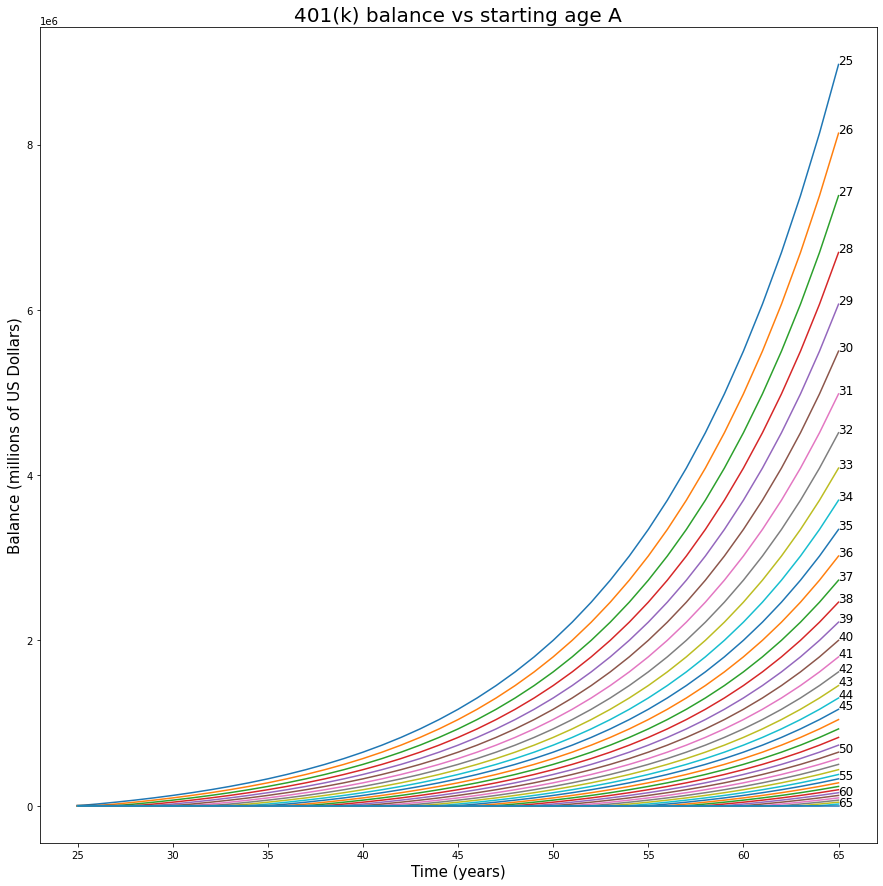
\includegraphics[scale=0.45]{hw10-q4-b.png}
		\end{solution}

		\part Obviously, the total quantity of money you have deposited at time $t$ is $M(t-A)$.
		Plot $b(R) / M(R-A)$ as a function of $A$ the age you start saving, assuming you retire at $R=65$.
		This ratio is your `bang-for-the-buck'.

		\begin{solution}

			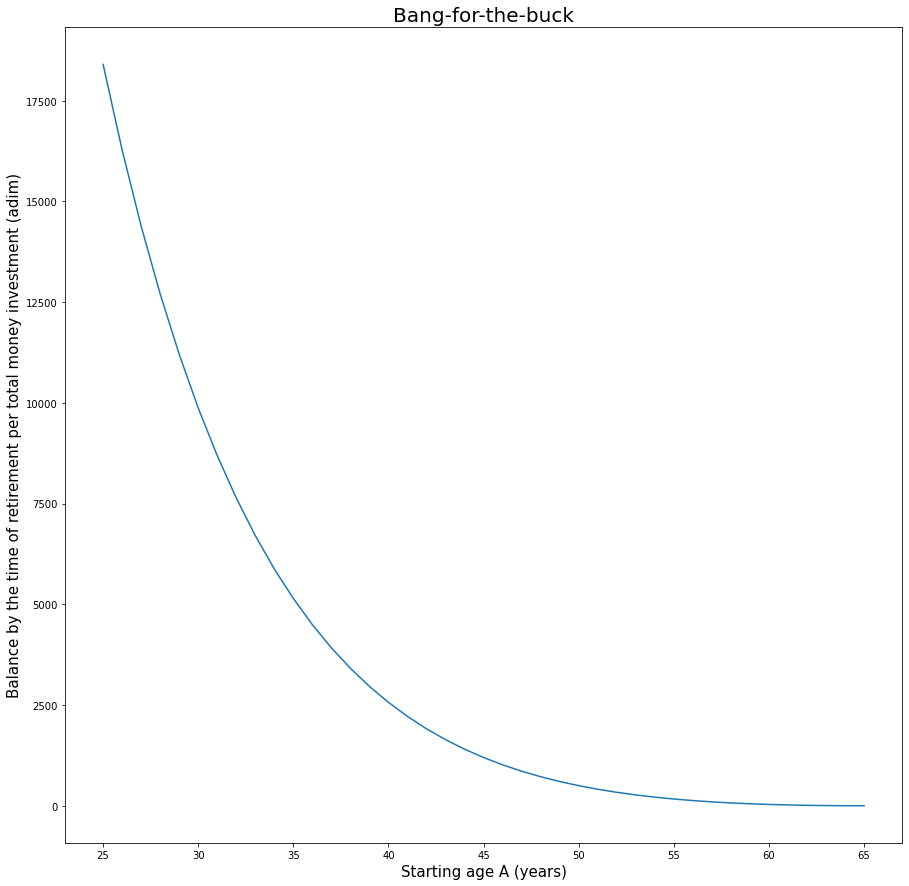
\includegraphics[scale=0.45]{hw10-q4-c.png}
		\end{solution}

		\part According to this naive model, how much more money will you save if you start saving at $A=25$ than if you start at $A=30$, assuming $R=65$?

		\begin{solution}
			Using the algorithm (annex), $$b(t=65,A=25) - b(t=65,A=30) = \textbf{US\$ }3,469,396.04.$$

		\end{solution}

	\end{parts}
	Reality check: the average American---especially the average 25-year-old---doesn't typically have a job where they can easily deposit the maximum $M$ into their 401(k)---it'd be too large a percentage of their take-home pay.
	So what happens more realistically is that the deposit rate $d$ starts out low and grows as you advance in your career.
	Don't feel stressed out if you don't get such a lucrative job at 25; the point of this question is to prepare you to understand the gist of the computation you must do to roughly understand your future; you can plug in more realistic functions!



	\section*{Solving ODEs with Laplace Transforms (using convolutions!)}
	\question Boas 8.12.5

	\begin{solution}
		``Obtain (12.6) by using the convolution integral to solve (12.1)."

		(12.1) is given by $y'' + \omega^2 y = f(t)$, $y_0 = y'_0 = 0$. Taking the laplace transform,

		$$ \stackrel{\mathcal{L}}{\rightarrow} k^2 Y - k y_0 - y'_0 + \omega^2 Y = F(k) $$
		$$ (k^2 + \omega^2) Y = F(k) $$
		$$ Y = \frac{F(k)}{(k^2 + \omega^2)} = F(k) \omega^{-1}  \frac{\omega}{(k^2 + \omega^2)}$$
		$$ \stackrel{\mathcal{L}^{-1}}{\rightarrow} y = f(t) \ast \omega^{-1} \sin \omega t = \frac{ f(t) \ast \sin \omega t }{\omega}$$
		$$ = \int_0^t \frac{1}{\omega} \sin \omega (t - \tau) f(\tau) \id{\tau}$$
		which is equation (12.6).

	\end{solution}

	\question Consider a system goverened by the ODE
	\begin{equation}
		\ddot{y} + 2b \dot{y} + \omega_0^2 y = f(t)
	\end{equation}
	which starts with $\dot{y}(0)=\dot{y}_0$ and $y(0)=y_0$.

	\begin{parts}
		\part Show that the Laplace transform of the ODE leads to
		\begin{equation}
			Y
			=
			\frac{F}{s^2+2bs+\omega_0^2} + \frac{s y_0}{s^2+2bs+\omega_0^2} + \frac{2 b y_0 + \dot{y}_0}{s^2+2bs+\omega_0^2}
		\end{equation}
		where $Y=\laplace{y}$ and $F=\laplace{f}$.
		
		\begin{solution}
			$$\stackrel{\mathcal{L}}{\rightarrow} s^2 Y - sy_0 - \dot{y_0} + 2b(sY - y_0) + \omega^2 Y= F(s)$$
			$$ (s^2 + 2bs + \omega^2) Y = F(s) + sy_0 + \dot{y_0} + 2by_0 $$
			$$ Y = \frac{F}{s^2 + 2bs + \omega^2} + \frac{sy_0}{s^2 + 2bs + \omega^2} + \frac{2by_0 + \dot{y_0}}{s^2 + 2bs + \omega^2}$$

		\end{solution}

		Let's stop and take this this form in for a second.  The first piece is the same no matter what the initial conditions are---it therefore corresponds to a particular solution.  The other two pieces have constants in them fixed by the initial conditions---they are part of the complementary function (remember?  the solution to the associated homogeneous equation?)

		\part Let's first consider $F=0$ with the above initial conditions so that we get the appropriate complementary function.  Assume were are not in the critically damped case.  Show that
		\begin{align}
			y_c   & = \oneover{2\sqrt{b^2-\omega_0^2}} \left[ \left(\dot{y}_0 - y_0r_-\right) e^{r_+ t} - \left(\dot{y}_0 - y_0r_+\right) e^{r_- t}\right] u(t)
			      &
			r_\pm & = -b \pm \sqrt{b^2-\omega_0^2}
		\end{align}
		where $r_\pm$ are the charactersitic roots of the equation (remember?!).
		Notice that this solution has the property that $y(0) = y_0$ and $\dot{y}(0) = \dot{y}_0$ it satisfied the ODE for all $t>0$; where we expect Laplace transform methods to work.
		\begin{solution}
			Suppose that $F = 0$ and $ b^2 \neq \omega^2$. Also, $s^2 + 2bs + \omega^2 = (s-r_-)(s-r_+)$ where $r = -b \pm \sqrt{b^2 - \omega_0^2}$.
			$$ Y_c = \frac{sy_0}{(s-r_-)(s-r_+)} + \frac{2by_0 + \dot{y_0}}{(s-r_-)(s-r_+)}$$
			$$ Y_c = y_0 \frac{s}{(s-r_-)(s-r_+)} + (2by_0 + \dot{y_0})\frac{1}{(s-r_-)(s-r_+)}$$
			Using L7 and L8 from Boas' Laplace table,
			$$ y_c = y_0 \left[ \frac{(-r_-)e^{r_- t} - (-r_+)e^{r_+ t}}{(-r_-) - (-r_+)} \right] + (2by_0 + \dot{y_0}) \left[ \frac{e^{r_- t} - e^{r_+ t}}{(-r_+) - (-r_-)} \right]$$
			$$ y_c = y_0 \left[ \frac{r_- e^{r_- t} - r_+ e^{r_+ t}}{r_- - r_+} \right] + (2by_0 + \dot{y_0}) \left[ \frac{e^{r_- t} - e^{r_+ t}}{r_- - r_+} \right]$$
			$$ y_c = \oneover{r_- - r_+} \left[ e^{r_- t} \left( y_0 r_- + 2by_0 + \dot{y_0} \right) - e^{r_+ t} \left(y_0 r_+ + 2by_0 + \dot{y_0}  \right)   \right]$$
			$$ y_c = \oneover{r_- - r_+} \left[ e^{r_- t} \left( y_0 (r_- + 2b) + \dot{y_0} \right) - e^{r_+ t} \left(y_0 (r_+ + 2b) + \dot{y_0})  \right)   \right]$$

			There's a subtlety here that $r_+ + 2b = - r_-$ and $r_- + 2b = - r_+$. 
			
			Also, $r_- - r_+ = -2\sqrt{b^2 - \omega_0^2}$. And thus,

			$$ y_c = \frac{-1}{2\sqrt{b^2 - \omega_0^2}} \left[ e^{r_- t} \left( y_0 (- r_+ ) + \dot{y_0} \right) - e^{r_+ t} \left(y_0 (-r_-) + \dot{y_0})  \right)   \right]$$
			$$ y_c = \frac{1}{2\sqrt{b^2 - \omega_0^2}} \left[ e^{r_+ t} \left(\dot{y_0} - y_0 r_-  \right) - e^{r_- t} \left(\dot{y_0} -y_0 r_+  \right)  \right] u(t) $$

			The $u(t)$ was added as a convention; since the Laplace erases the function for $t<0$, we can't have any information on that domain after we take the inverse laplace.

		\end{solution}

		\part Show that
		\begin{equation}
			W(t) = \inverselaplace{\oneover{s^2+2bs+\omega_0^2}} = \oneover{2\sqrt{b^2-\omega_0^2}} \left[ e^{r_+ t} - e^{r_- t}\right] u(t),
		\end{equation}
		again assuming we're not in the critical case.  (You can probably re-use some of the partial-fractions from the previous part, if that's how you did it.)

		\begin{solution}
			
			$$\oneover{s^2+2bs+\omega_0^2} = \frac{1}{(s-r_-)(s-r_+)} = \frac{A}{s-r_-} + \frac{B}{s-r_+}$$
			$$ 1 = A(s-r_+) + B(s-r_-) = s(A+B) - A r_+ - B r_- $$
			$$ \Rightarrow B = -A \Rightarrow - A r_+ - B r_- = A (r_- - r_+) = 1$$
			$$ \Rightarrow A = \frac{-1}{2 \sqrt{b^2 - \omega_0^2}}\textbf{,  } B = \frac{1}{2 \sqrt{b^2 - \omega_0^2}}$$
			Thus,
			$$\oneover{s^2+2bs+\omega_0^2} = \frac{1}{2 \sqrt{b^2 - \omega_0^2}} \left[ \frac{1}{s-r_+} - \frac{1}{s-r_-} \right] $$
			Taking the inverse laplace (L2 from the table),
			$$W(t) = \oneover{2\sqrt{b^2-\omega_0^2}} \left[ e^{r_+ t} - e^{r_- t}\right] u(t)$$

		\end{solution}

		\part Now you know the general solution to the ODE for any $f(t)$---just convolve $W*f$ to find the particular solution and add the complementary solution.
		Try it for a delta-function impulse at time $t_i>0$ $f = f_i \delta(t-t_i)$.
		Show that the particular solution
		\begin{equation}
			y_p = W*f = \frac{e^{r_+-(t-t_i)} - e^{r_-(t-t_i)}}{r_+-r_-} f_i u(t-t_i)
		\end{equation}
		by directly evaluating the convolution integral $W*f = \int_0^{t} \id{\tau}\; W(\tau) f(t-\tau)$.
		You might want to consider two cases: $t<t_i$ and $t>t_i$ separately, as shown for the question on nuclear dumping.
		Notice that the particular solution only `kicks in' once the system receives the impulse---that makes physical sense!
		Also---what is the behavior?
		It's exactly what you expect---decaying exponentially (there are decaying oscillations if we're in the underdamped case).
		
		\begin{solution}
			So $f = f_i \delta(t-t_i)$. Let's compute the above convolution:
			$$  y_p = W\ast f = \int_0^t \oneover{2\sqrt{b^2-\omega_0^2}} \left[ e^{r_+ \tau} - e^{r_- \tau}\right] u(\tau) f_i \delta(\tau - (t - t_i)) \id{\tau}  $$
			$$ = \frac{f_i}{2\sqrt{b^2-\omega_0^2}} \left[ e^{r_+ (t-t_i)} - e^{r_- (t-t_i)}\right] u(t-t_i)$$
			$$ = \frac{e^{r_+-(t-t_i)} - e^{r_-(t-t_i)}}{r_+-r_-} f_i u(t-t_i)$$
		\end{solution}

	\end{parts}
	In class we mentioned that the $\delta$ is the identity element for the convolution operation, $\delta*g = g*\delta = g$ for any $g$.  We also mentioned that convolution is associative, $(a*b)*c = a*(b*c)$, because the Laplace transform of both sides is $ABC$.
	Suppose we have some other signal, not $f(t) = \delta(t)$ (setting $t_i=0$ and $f_i=1$) but $g(t)$.  The particular solution given $f$ is $f*W = \delta*W = y_p$.  Since $g= g*\delta$ the particular solution for $g$ as input is $(g*\delta)*W = g*(\delta*W) = g*y_p$ where $y_p$ is what we just found (with $t_i=0$ and $f_i=1$ plugged in---which is $W$ itself!).
	The whole thing hangs together!
	\section*{As Always}
	\question How long did this problem set take you? About 7 hours.

	\section*{Optional Practice}

	\question Boas 8.10.1
	\question Boas 8.10.2
	\question Boas 8.10.{3-12} are good practice for using the table or for applying partial fractions decomposition.
	\question Boas 8.10.13
	\question Boas 8.10.{14,15} for practice solving differential equations.
	\question Boas 8.10.17; you can also try it with $+a^2$ instead of $-a^2$.
\end{questions}

\end{document}
